%=======================================================================
%  Volatility Forecasting in an Unregulated Retail Asset Market
%  Evidence from the Counter-Strike 2 skin market
%
%  Compiles as-is on Overleaf (pdfLaTeX). No external .bib needed.
%=======================================================================
\documentclass[11pt,a4paper]{article}

\usepackage[utf8]{inputenc}
\usepackage[T1]{fontenc}
\usepackage{lmodern}
\usepackage{amsmath,amssymb}
\usepackage{booktabs}
\usepackage{multirow}
\usepackage{graphicx}
\usepackage{geometry}
\usepackage{natbib}
\usepackage{hyperref}
\usepackage{caption}

\geometry{margin=1in}
\bibliographystyle{plainnat}
\setcitestyle{authoryear,round}
\hypersetup{colorlinks=true,linkcolor=blue,citecolor=blue,urlcolor=blue}

\title{\textbf{Volatility Forecasting in an Unregulated Retail Asset Market:}\\[0.3em]
\large Evidence from the Counter-Strike 2 Skin Market}

\author{Sayed Mohammad Nasrullah Bin Mohd Noor\\
\small University of Manchester}

\date{\today}

\begin{document}
\maketitle

\begin{abstract}
\noindent
We study volatility dynamics in the Counter-Strike 2 (CS2) skin market, a
multi-billion-dollar retail asset market that lacks market makers, arbitrageurs,
short selling and circuit breakers, and in which a single agent controls supply
by decree. Using daily median prices for 24 items over 2021--2026, we document
the following. First, returns exhibit genuine ARCH effects (22 of 24 items) but
also a \emph{predictable conditional mean} (24 of 24 items), a property that is
almost absent from equity returns and which we interpret as direct evidence of
missing arbitrage capital. The predictability is partly seasonal: returns
display a weekly cycle, with mean returns ranging from $-0.64\%$ on Wednesdays
to $+0.40\%$ on Saturdays. Second, fitted GARCH persistence does not scale with
item value, contradicting a gradient visible in raw absolute-return
autocorrelations; the discrepancy is a caution about proxy choice rather than a
substantive finding. Third, and centrally, \emph{no estimated GARCH-family
specification significantly outperforms a parameter-free benchmark on any item}
in out-of-sample one-day-ahead forecasting, evaluated with QLIKE and
Diebold--Mariano tests. An exponentially weighted moving average lies inside
the 90\% Model Confidence Set on every item and is the sole survivor on five,
while every estimated specification is excluded on seven. EGARCH, which wins
BIC in-sample on half the panel, ranks last out of sample. The result is robust
across a sixteen-fold range of EWMA smoothing constants and across four
cleaning specifications. We argue that volatility in this market carries too
little stable structure to justify estimating conditional variance parameters.
The paper appears to be the first formal out-of-sample evaluation of volatility
forecasts in a virtual asset market.

\medskip
\noindent\textbf{Keywords:} volatility forecasting, GARCH, virtual economies,
QLIKE, Diebold--Mariano, retail markets

\noindent\textbf{JEL:} C22, C53, G17, L86
\end{abstract}

%=======================================================================
\section{Introduction}
%=======================================================================

Most of what is known about conditional volatility comes from markets with
professional intermediation. Equity, foreign exchange and commodity markets
have market makers who quote two-sided prices, arbitrageurs who eliminate
predictable returns, short sellers who can express negative views, and
exchange-level circuit breakers that interrupt disorderly trading. Volatility
models of the GARCH family \citep{Engle1982,Bollerslev1986} were developed
against this institutional backdrop, and the stylised facts they are designed
to capture---clustering, fat tails, leverage---were established there.

This paper asks what conditional volatility looks like, and whether it can be
forecast, when that machinery is absent. The setting is the market for
cosmetic weapon skins in Counter-Strike 2 (CS2), traded on the Steam Community
Market. The market has several properties that make it a useful laboratory:

\begin{itemize}
\item \textbf{No intermediation.} Trades are peer-to-peer. There are no market
makers, no designated liquidity providers, and no institutional capital.
\item \textbf{No short selling and no derivatives.} A negative view can only be
expressed by selling inventory one already owns.
\item \textbf{High frictions.} Steam charges roughly 15\% per transaction
\citep{Dobrynskaya2025}, which makes short-horizon arbitrage uneconomic even
where price predictability exists.
\item \textbf{Retail-only participation.} Holders are overwhelmingly players
and small speculators.
\item \textbf{Centralised, discretionary supply.} Valve, the game's publisher,
can alter the supply of any item---or the mechanism by which items are
produced---without notice, consultation or compensation.
\end{itemize}

\noindent
The paper proceeds in four parts. Section~\ref{sec:facts} documents the
distributional and dependence properties of daily skin returns, including the
predictable conditional mean that distinguishes this market sharply from
equities, a weekly seasonal cycle, and the coexistence of two opposing
microstructure signatures at different points of the price distribution.
Section~\ref{sec:models} estimates AR(7)-GARCH, EGARCH and GJR-GARCH
specifications with Student-$t$ errors and shows that volatility persistence
does not vary systematically with item value---a negative result that
contradicts a gradient visible in a naive proxy.
Section~\ref{sec:forecast} is the core of the paper: in out-of-sample
one-day-ahead forecasting, no estimated specification beats a parameter-free
benchmark on any item, a result that survives Model Confidence Set testing and
sensitivity analysis over both the smoothing constant and the cleaning
procedure. Section~\ref{sec:shock} asks whether any specification withstands
an exogenous structural break.

That last finding places the paper in the tradition of \citet{HansenLunde2005},
who compared 330 ARCH-type models and found no evidence that any outperformed
a plain GARCH(1,1) on exchange rate data. Our result is stronger in one
direction and weaker in another: stronger because \emph{nothing estimated}
beats a benchmark with no free parameters at all, weaker because our volatility
proxy is the squared daily return rather than realised variance. We address
the proxy problem by following \citet{Patton2011} and using QLIKE, whose
forecast ranking is robust to noise in the proxy, as the primary loss function.

%=======================================================================
\section{Related literature}
%=======================================================================

\paragraph{Microstructure in thin markets.}
Both of the dependence patterns documented in Section~\ref{sec:facts} have
established microstructure explanations. \citet{Roll1984} shows that
alternation between buyer- and seller-initiated trades induces negative
first-order autocorrelation in transaction returns, with
$\mathrm{Cov}(r_t, r_{t-1}) = -s^2/4$ for effective spread $s$; the effect
dominates the return series where percentage spreads are wide.
\citet{ScholesWilliams1977} and \citet{LoMacKinlay1990} analyse the opposite
case, in which non-synchronous or infrequent trading carries stale prices
forward and induces \emph{positive} serial correlation. Both mechanisms are
present in our panel, on different items.
\citet{LamoureuxLastrapes1990} show that unmodelled shifts in unconditional
variance generate spurious persistence in GARCH estimates, which bears
directly on the boundary solutions reported in Section~\ref{sec:models}.

\paragraph{Virtual asset markets.}
A small but growing literature treats videogame items as financial assets.
\citet{Dobrynskaya2025} study monthly returns on 4{,}565 CS:GO skins over
2013--2024 and find average returns of roughly 40\% per annum, low correlation
with equity risk factors, and pronounced seasonality with peaks in January and
April. \citet{Glaser2022} documents how Valve, as platform owner, shapes market
infrastructure and pricing mechanisms. Closest to our setting,
\citet{Gu2026} analyses the CS:GO/CS2 market over 2022--2024, applying the
\citet{Amihud2002} illiquidity measure to butterfly knives to show that
crashes in this market are characterised by liquidity evaporation rather than
high-volume selling, treating the 2025 Trade-Up policy change as a brief
out-of-sample extension. \citet{Nian2026} applies event-study methodology to
CS:GO skin prices around Valve announcements.

The published work above studies \emph{returns}---their level, their
cross-section, their risk exposures---or \emph{liquidity} around a single
event. We are not aware of any peer-reviewed study of the forecastability of
conditional variance in a virtual asset market. The question of whether
standard volatility technology transfers to a market without professional
intermediation is separate from, and not answered by, the finding that skins
earn high average returns.

The closest antecedent is an unpublished working paper. \citet{Nikolaenko2025}
fits ARMA--GARCH(1,1) specifications to two CS:GO skins, tests for
stationarity and structural breaks, and computes rolling one-step-ahead
conditional variance forecasts, concluding that predictive power is weak. Our
paper differs in three respects that we regard as material. First, scope:
twenty-two items stratified across four price tiers rather than two. Second,
and centrally, evaluation---forecasts here are scored against parameter-free
benchmarks using proxy-robust loss functions, with Diebold--Mariano tests and a
Model Confidence Set, so that ``weak predictive power'' becomes a testable
comparative claim rather than a qualitative impression. Third, we exploit the
October 2025 Trade-Up policy change as an identified structural break rather
than treating breaks solely as a nuisance for stationarity testing.

One substantive disagreement is worth recording. \citet{Nikolaenko2025}
reports little autocorrelation in skin returns, whereas we reject the null of
no autocorrelation on every item in our panel (Section~\ref{sec:facts}). The
discrepancy is most plausibly one of sample breadth---two items against
twenty-four---but it may also reflect our longer window or the weekly seasonal
documented below, which a short sample would struggle to detect. We note that
one item, M4A1-S $\vert$ Decimator, appears in both panels.

\paragraph{Volatility model comparison.}
\citet{HansenLunde2005} is the canonical reference for the proposition that
elaborate volatility specifications rarely improve on simple ones out of
sample; \citet{HLN2011} provide the Model Confidence Set, which formalises
the question of whether any model can be statistically distinguished from the
best. The recurring empirical pattern across asset classes is that simple
benchmarks---exponentially weighted averages, or realised-volatility
averages---remain inside the confidence set, and that added structure yields
marginal gains at best. Our result is a strong form of this: in a market with
high microstructure noise, thin trading and retail dominance, the
parameter-free benchmark is not merely competitive but strictly better. \citet{Patton2011} establishes the conditions under which a loss
function ranks volatility forecasts consistently despite an imperfect proxy,
and identifies QLIKE and MSE as the two leading robust members of that class.
\citet{DieboldMariano1995} provides the test of equal predictive accuracy used
throughout. \citet{AndersenBollerslev1998} established that daily squared
returns, while conditionally unbiased, are an extremely noisy volatility
proxy, and that intraday realised measures track conditional variance far more
closely---a benchmark unavailable here, and the principal methodological
limitation of this paper. On specifications, we use \citet{Bollerslev1986} for GARCH,
\citet{Nelson1991} for EGARCH and \citet{Glosten1993} for the threshold
(GJR) form, with \citet{RiskMetrics1996} supplying the exponentially weighted
benchmark.

%=======================================================================
\section{Data}\label{sec:data}
%=======================================================================

\subsection{Source and sample construction}

Prices come from the Steam Community Market price history endpoint for
application 730 (CS2), which returns, for each item, the median transaction
price and the number of units sold. Observations arrive hourly for
approximately the trailing thirty days and daily thereafter; we aggregate
everything to daily frequency before constructing returns, since a series that
is hourly at its tail and daily elsewhere would produce a spurious volatility
regime shift at the joint. Prices are denominated in Malaysian ringgit, the
currency of the querying account; because log returns are scale-free this
affects only the price-tier labels used for stratification.

Item selection proceeds in two stages, deliberately separated. First, a
\emph{discovery} stage enumerates the market by scanning 6{,}000 listings
sorted by price descending and 1{,}000 sorted by listing count, retaining the
forty most-listed items within each of four price tiers. Neither sort is a
quality judgement: sorting by listing count alone returns almost exclusively
cheap weapon cases, while sorting by price alone returns knives that trade only
a few times per month. Second, a \emph{screening} stage selects on realised
trading activity rather than on listing metadata, requiring at least 500
observations, median daily volume of at least five units, and no more than 5\%
missing days. Of 160 candidates, 111 pass; these are stratified across price
tier and item category to yield a working panel of 29.

\subsection{Data quality}

Three distinct problems were identified by inspection and are handled
explicitly.

\paragraph{Stale pricing.} Two sticker items printed an identical median price
on approximately 75\% of days. A return series dominated by exact zeros will
still yield GARCH estimates, but the implied persistence is an artefact of
quantisation. Both items were dropped.

\paragraph{Penny items.} Below roughly RM~0.50 the median price is quantised to
a handful of ticks and can be displaced for several consecutive days by a small
number of trades. Three items were dropped on this basis; mean annualised
volatility in the cheapest tier fell from 5.06 to 0.75 as a result, which
indicates how severely these observations distorted the tier.

\paragraph{Isolated bad prints.} The Steam median occasionally reports a price
orders of magnitude away from trend for exactly one day before reverting. One
item priced around RM~2{,}200 printed RM~11.74 on a single day. Because a
genuine price move persists while a bad print reverses, we repair only those
observations for which $|r_t| > 0.8$ and $|r_t + r_{t+1}| < 0.35|r_t|$,
replacing the price with the geometric mean of its neighbours. Seventy-five
observations across seven items were repaired. Mean excess kurtosis in the
most expensive tier fell from 217 to 9.3.

We stress that the repair filter is deliberately narrow. The largest price
movements in the sample are \emph{not} errors: on 23 October 2025 two items in
the panel rose by more than 370\% and three fell by 29--43\%, and these moves
persisted. Any filter aggressive enough to remove that episode would be
removing the most economically informative observations in the data. This is
discussed in Section~\ref{sec:shock}.

The final panel comprises 24 items and 54{,}380 daily returns. Two further
items are held out of the main analysis for reasons given in
Section~\ref{sec:facts}, leaving 22 for estimation and 21 for forecasting.

%=======================================================================
\section{Stylised facts}\label{sec:facts}
%=======================================================================

Diagnostics are run before any model is fitted. This ordering matters: a GARCH
model will converge and report parameters whether or not conditional
heteroskedasticity is present, so the presence of ARCH effects must be
established independently rather than assumed.

Let $r_t = \log(P_t) - \log(P_{t-1})$ denote the daily log return. We compute
Ljung--Box statistics on $r_t$ and $r_t^2$ at ten lags, the ARCH-LM test of
\citet{Engle1982}, and the Jarque--Bera normality test. Results are summarised
in Table~\ref{tab:facts}.

\begin{table}[htbp]
\centering
\caption{Stylised facts, 2021--2026, 24 items}
\label{tab:facts}
\begin{tabular}{lc}
\toprule
Property tested & Items \\
\midrule
Volatility clusters (Ljung--Box on $r_t^2$, $p<0.05$) & 22 / 24 \\
ARCH effects present (ARCH-LM, $p<0.05$)             & 22 / 24 \\
Returns non-normal (Jarque--Bera, $p<0.05$)          & 24 / 24 \\
Conditional mean unpredictable (Ljung--Box on $r_t$, $p\geq0.05$) & 0 / 24 \\
\bottomrule
\end{tabular}
\end{table}

Annualised volatility ranges from 44\% to 224\%, against roughly 15--20\% for
the S\&P~500 over comparable periods, with excess kurtosis in the tens.
Figure~\ref{fig:clustering} shows the characteristic clustering directly, and
Figure~\ref{fig:tails} confirms that the tails are far heavier than Gaussian
in both directions.

\begin{figure}[htbp]
\centering
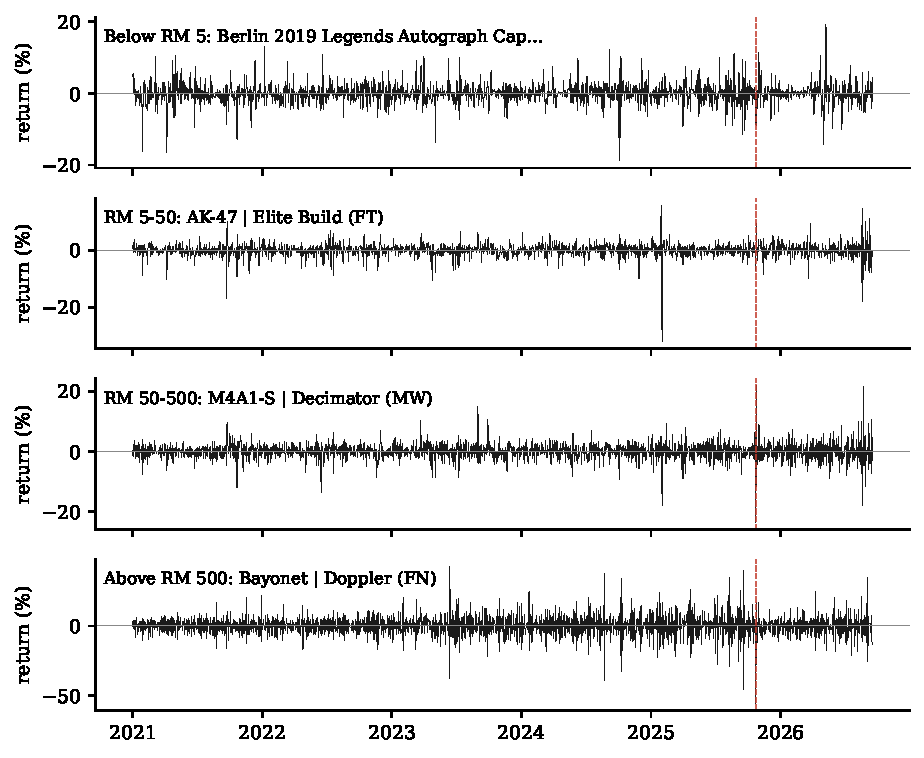
\includegraphics[width=\textwidth]{figures/fig1_clustering}
\caption{Daily returns for one representative item in each price tier,
2021--2026. The dashed vertical line marks 23 October 2025. Volatility
clustering is visible in every tier.}
\label{fig:clustering}
\end{figure}

\begin{figure}[htbp]
\centering
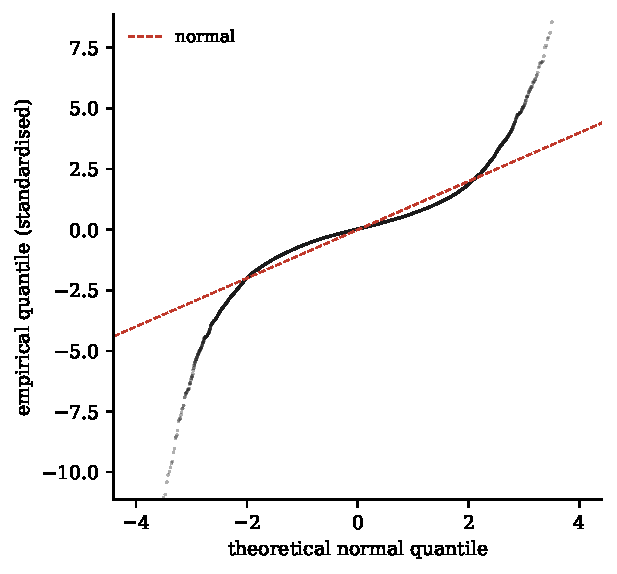
\includegraphics[width=0.62\textwidth]{figures/fig3_tails}
\caption{Quantile--quantile plot of pooled standardised returns against the
normal distribution. Deviation is severe and symmetric in both tails.}
\label{fig:tails}
\end{figure}

\paragraph{The predictable mean.}
The final row of Table~\ref{tab:facts} is the most substantively interesting
result in this section. Ljung--Box rejects the null of no autocorrelation in
raw returns for \emph{every} item in the panel. Equity returns essentially
never display this at daily frequency, because predictable returns invite
arbitrage and arbitrage eliminates them. Here there is no capital to do the
eliminating, and transaction costs of roughly 15\% would in any case make
exploitation uneconomic at the magnitudes involved. The predictable mean is
therefore not a nuisance to be differenced away but direct evidence of the
market's institutional structure. It also implies that a constant-mean
specification is misspecified, and motivates the autoregressive mean used
throughout Section~\ref{sec:models}.

\paragraph{A weekly cycle.}
Figure~\ref{fig:acf} decomposes the dependence structure. The right panel
shows the expected pattern for squared returns: strong positive autocorrelation
decaying over roughly ten days. The left panel is the unusual one. First-order
autocorrelation is significant on 21 of 24 items and pronounced spikes appear
at lags 7 and 14, with lag-7 autocorrelation individually significant on 10 of
24 items and a panel mean of $+0.086$.

\begin{figure}[htbp]
\centering
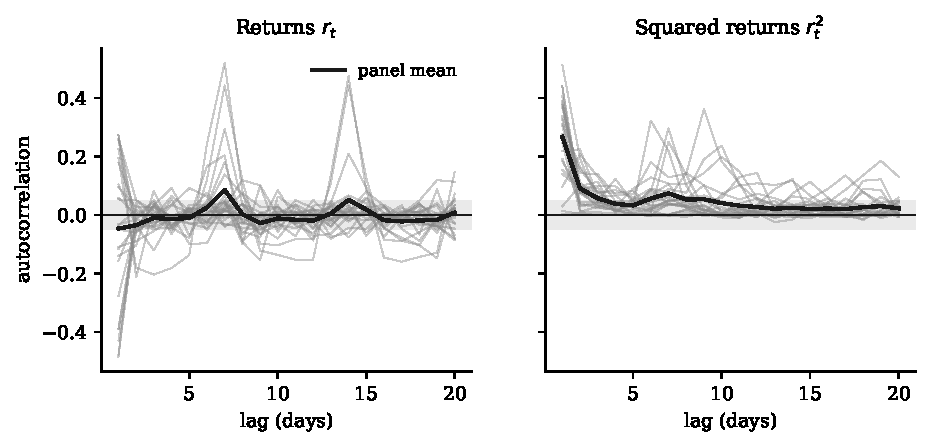
\includegraphics[width=\textwidth]{figures/fig2_acf}
\caption{Sample autocorrelation of returns (left) and squared returns (right).
Grey lines are individual items; the heavy line is the panel mean; the shaded
band is the approximate 95\% interval under no autocorrelation. Note the
spikes at lags 7 and 14 in the left panel.}
\label{fig:acf}
\end{figure}

This is a weekly seasonal. Pooled mean returns by weekday range from $-0.64\%$
on Wednesdays to $+0.40\%$ on Saturdays. The interpretation is
straightforward and not financial: participation in this market follows player
activity, which concentrates at weekends, and with no professional traders to
smooth the resulting order flow the cycle survives into prices.
\citet{Dobrynskaya2025} document monthly seasonality in the same market with
peaks in January and April; the weekly cycle appears to be the daily-frequency
analogue. It also dictates the mean specification used below.

\paragraph{Two microstructure regimes.}
The panel mean first-order autocorrelation of $-0.046$ conceals a split. Of the
21 items with significant $\rho_1$, eleven are negative and ten positive, and
the sign is almost entirely determined by price tier
(Table~\ref{tab:rho1}).

\begin{table}[htbp]
\centering
\caption{First-order autocorrelation and implied Roll spread by price tier}
\label{tab:rho1}
\begin{tabular}{lcccc}
\toprule
Price tier & Items & Mean $\rho_1$ & Roll spread (\%) & Spread / daily vol. \\
\midrule
Below RM 5   & 6  & $+0.186$ & --- & --- \\
RM 5--50     & 10 & $-0.016$ & 2.97 & 0.65 \\
RM 50--500   & 3  & $-0.003$ & 2.18 & 0.79 \\
Above RM 500 & 5  & $-0.412$ & 11.04 & 1.28 \\
\bottomrule
\end{tabular}
\end{table}

High-value items display strongly negative $\rho_1$, the signature of
bid--ask bounce \citep{Roll1984} in a market where percentage spreads are
wide. Inverting the Roll relation gives implied effective spreads of 11\% for
knives against roughly 3\% at mid tier, economically plausible alongside
Steam's 15\% transaction fee. Two caveats apply. The Roll measure is undefined
where $\rho_1 > 0$, which excludes 11 of 24 items, and the implied spread
correlates 0.97 with daily volatility because it scales with $\sigma$
mechanically. Normalising by volatility preserves the ordering (final column),
so a genuine spread gradient exists, but the raw magnitudes should not be read
as pure spread estimates.

Cheap items show the opposite sign. Positive serial correlation is the
signature of non-synchronous or stale pricing
\citep{ScholesWilliams1977,LoMacKinlay1990}: where a median price updates only
on days with sufficient trade, prices are carried forward and returns are
smoothed. The same market therefore exhibits both classical microstructure
patterns simultaneously, separated by item value---plausibly because expensive
items trade rarely at wide spreads while cheap items trade often at prices that
barely move.

\paragraph{Two items held out.}
Two items---AWP $\vert$ Chromatic Aberration (Field-Tested) and
AK-47 $\vert$ Head Shot (Field-Tested)---return ARCH-LM $p$-values of
approximately 1.0 and excess kurtosis near 490. This is not an absence of
conditional heteroskedasticity but its opposite: a single return of $+378\%$
and $+394\%$ respectively on 23 October 2025 so dominates the squared-return
series that no test can detect clustering around it. Both are excluded from
Sections~\ref{sec:models} and~\ref{sec:forecast} and analysed separately in
Section~\ref{sec:shock}. We prefer exclusion to an event dummy because a dummy
requires defending a particular parameterisation of a shock whose magnitude is
unprecedented in the sample.

%=======================================================================
\section{Models and estimation}\label{sec:models}
%=======================================================================

\subsection{Specifications}

The mean equation is AR(7) for all items and all specifications:
\begin{equation}
r_t = \mu + \sum_{j=1}^{7} \phi_j r_{t-j} + \varepsilon_t,
\qquad \varepsilon_t = \sigma_t z_t,
\qquad z_t \sim t_\nu .
\end{equation}

Seven lags are used to accommodate the weekly cycle documented in
Section~\ref{sec:facts}; the lag-7 coefficient carries most of the
explanatory content. Table~\ref{tab:mean} compares the alternatives.

\begin{table}[htbp]
\centering
\caption{Mean specification comparison, 22 items, GARCH(1,1)-$t$ variance}
\label{tab:mean}
\begin{tabular}{lcccc}
\toprule
Mean model & Mean BIC & Mean log-lik. & Residual ACF(7) & Lowest BIC \\
\midrule
Constant & 8370.3 & $-4166.9$ & $+0.092$ & 1 / 22 \\
AR(1)    & 8276.7 & $-4116.5$ & $+0.099$ & 3 / 22 \\
AR(7)    & \textbf{8139.3} & $\mathbf{-4025.9}$ & $-0.044$ & \textbf{18 / 22} \\
\bottomrule
\end{tabular}
\end{table}

AR(7) attains lowest BIC on 18 of 22 items and reduces residual lag-7
autocorrelation from $+0.099$ to $-0.044$. Residual weekly autocorrelation
nonetheless remains significant on 13 of 22 items, so the specification
improves on but does not fully resolve the seasonal.

We hold the mean specification fixed across items rather than selecting per
item. Per-item selection would leave variance parameters estimated under
different mean structures and hence not comparable across the cross-section,
which is the dimension of interest.

The variance equations are
\begin{align}
\text{GARCH(1,1):}\quad
&\sigma_t^2 = \omega + \alpha \varepsilon_{t-1}^2 + \beta \sigma_{t-1}^2 \\[0.3em]
\text{GJR-GARCH(1,1):}\quad
&\sigma_t^2 = \omega + \alpha \varepsilon_{t-1}^2
 + \gamma \varepsilon_{t-1}^2 I_{\{\varepsilon_{t-1}<0\}} + \beta \sigma_{t-1}^2 \\[0.3em]
\text{EGARCH(1,1):}\quad
&\log \sigma_t^2 = \omega
 + \alpha \left( |z_{t-1}| - \mathbb{E}|z_{t-1}| \right)
 + \gamma z_{t-1} + \beta \log \sigma_{t-1}^2
\end{align}

Student-$t$ innovations are used throughout, with Gaussian GARCH estimated
alongside as a comparison. Two benchmarks complete the set: exponentially
weighted moving average (EWMA), $\sigma_t^2 = \lambda \sigma_{t-1}^2
+ (1-\lambda)\varepsilon_{t-1}^2$ with $\lambda = 0.94$ following
\citet{RiskMetrics1996}, and a thirty-day rolling standard deviation. Neither
benchmark estimates any parameter from the data.

\subsection{Estimation results}

All 88 fits (22 items $\times$ 4 specifications) converge. Student-$t$
dominates Gaussian on every item, typically by 250--370 points of
log-likelihood. Estimated degrees of freedom range from 2.61 to 5.92 with a
median of 3.43; since the kurtosis of a Student-$t$ is undefined for
$\nu \leq 4$ and its skewness for $\nu \leq 3$, moment-based interpretation of
the fitted error distribution is not available. Standardised residual
kurtosis remains between 6 and 8, indicating that the $t$ absorbs most but not
all of the tail behaviour.

\paragraph{Persistence does not scale with item value.}
Our prior, formed from first-order autocorrelations of absolute returns
(0.41 in the most expensive tier against 0.20 in the mid tier), was that
high-value items would display greater volatility persistence, on the reasoning
that they are held disproportionately by speculators rather than players.
Fitted GARCH parameters do not support this (Table~\ref{tab:persist}).

\begin{table}[htbp]
\centering
\caption{Mean GARCH(1,1)-$t$ persistence $(\alpha+\beta)$ by price tier}
\label{tab:persist}
\begin{tabular}{lccc}
\toprule
Price tier & Items & All fits & Excluding boundary fits \\
\midrule
Below RM 5      & 6  & 0.970 & 0.939 \\
RM 5--50        & 10 & 0.880 & 0.829 \\
RM 50--500      & 1  & 0.891 & 0.891 \\
Above RM 500    & 5  & 0.878 & 0.797 \\
\bottomrule
\end{tabular}

\medskip
\begin{minipage}{0.92\textwidth}
\footnotesize Tier counts differ from Table~\ref{tab:rho1} because the two
items held out in Section~\ref{sec:facts} both fall in the RM 50--500 tier,
reducing it from three items to one.
\end{minipage}
\end{table}

The ordering is, if anything, the reverse of the hypothesis: the cheapest tier
is the most persistent. It is worth noting that \citet{Dobrynskaya2025} report
a ``penny stock effect'' in the same market, whereby cheaper skins earn higher
percentage returns. These are different moments of the same distribution and
the parallel is suggestive rather than evidential, but both point towards the
low-price segment behaving distinctly. We regard our result as a
methodological one rather than an economic one: absolute-return
autocorrelation is a raw statistic sensitive to outliers and level shifts,
while $\alpha+\beta$ is a conditional estimate that is not, and the apparent
gradient does not survive proper estimation. With as few as one item in a tier,
no claim in either direction is well powered.

\paragraph{Boundary solutions.}
Eight of 22 GARCH-$t$ fits return $\alpha+\beta$ of exactly 1.000. This is the
stationarity constraint binding rather than an estimate: at the boundary the
unconditional variance does not exist and standard errors are not valid. The
incidence is itself informative, but its interpretation is not straightforward:
\citet{LamoureuxLastrapes1990} show that unmodelled shifts in unconditional
variance produce exactly this appearance of near-integrated volatility, and our
sample contains at least one such shift. Whether these items genuinely exhibit
integrated volatility or merely unmodelled regime change cannot be settled
here. EGARCH does not suffer this, because
the log-variance formulation imposes no positivity constraint; its $\beta$ lies
between 0.58 and 0.98 on the same eight items. EGARCH-$t$ attains lowest BIC on
11 of 22 items, GARCH-$t$ on 9, and GJR-$t$ on 2.

\paragraph{Containers resist the model.}
Three items---two weapon cases and one key---leave significant ARCH effects in
standardised residuals under every specification tested. All three are
containers whose supply Valve controls directly through discrete injection
events. We report rather than drop them: the natural reading is that their
variance dynamics are driven by scheduled supply interventions and are
therefore not GARCH-shaped in the first place.

%=======================================================================
\section{Forecast evaluation}\label{sec:forecast}
%=======================================================================

\subsection{Design}

Forecasts are one-day-ahead, generated from a rolling 500-day estimation window
with weekly re-estimation, over 21 items and 119{,}425 forecast--realisation
pairs. A rolling rather than expanding window is used because the market
exhibits regime shifts, and an expanding window would carry stale pre-shock
observations indefinitely. Every forecast is genuinely out of sample: the
parameter vector used to forecast $\sigma_{t+1}^2$ is estimated on data through
$t$ only.

EGARCH occasionally converges to degenerate solutions producing variance
forecasts in excess of $10^{30}$. Because re-estimation is weekly, one such fit
would otherwise propagate for seven days and contaminate every loss average.
We therefore reject any re-estimation whose one-step forecast lies outside a
band of $[\bar{\sigma}^2/50,\; 50\bar{\sigma}^2]$ around the training-sample
variance, retaining the previous parameter vector instead. Fifty-one
re-estimations were rejected on this basis, all of them EGARCH; no other
specification produced any. We report this as a property of the specification
on this data rather than suppressing it.

\subsection{Loss functions}

Because no intraday data is available from the Steam endpoint, the realised
volatility proxy is the squared daily return $r_{t}^2$: conditionally unbiased,
but noisy. \citet{Patton2011} shows that under such a proxy the ranking induced
by a loss function need not be consistent for the true conditional variance
unless the loss belongs to a particular robust class. We therefore use QLIKE
as the primary loss,
\begin{equation}
L_{\text{QLIKE}}(\hat{\sigma}^2_t, r_t^2)
= \log \hat{\sigma}^2_t + \frac{r_t^2}{\hat{\sigma}^2_t},
\end{equation}
and report MSE, $L_{\text{MSE}} = (r_t^2 - \hat{\sigma}^2_t)^2$, for
comparability with the earlier literature. Where the two disagree, QLIKE is
preferred. Equal predictive accuracy is tested with
\citet{DieboldMariano1995}, using \citet{NeweyWest1987} standard errors on the
loss differential and the small-sample correction of \citet{Harvey1997}.

\subsection{Results}

\begin{table}[htbp]
\centering
\caption{Out-of-sample forecast performance, 21 items}
\label{tab:losses}
\begin{tabular}{lccc}
\toprule
Model & Mean QLIKE & Mean MSE & Items won (QLIKE) \\
\midrule
EWMA ($\lambda = 0.94$)  & \textbf{3.81} & \textbf{19{,}625} & \textbf{19} \\
Rolling SD (30 day)      & 3.91 & 20{,}305 & 1 \\
GARCH(1,1)-$t$           & 4.01 & 22{,}243 & 1 \\
GJR-GARCH(1,1)-$t$       & 4.02 & 22{,}513 & 0 \\
EGARCH(1,1)-$t$          & 4.10 & 51{,}310 & 0 \\
\bottomrule
\end{tabular}
\end{table}

Table~\ref{tab:losses} reports the central result. Under Diebold--Mariano at
the 5\% level, \emph{each of EGARCH-$t$, GARCH-$t$ and GJR-$t$ beats the
rolling standard deviation benchmark on zero of 19 items, and loses to it on
four to five}. EWMA beats the benchmark on 12 of 19 and loses on none; it beats
each estimated specification on 7 of 19 and loses to none.

\paragraph{The in-sample / out-of-sample reversal.}
EGARCH-$t$ attains lowest BIC in sample on 11 of 22 items and ranks last out of
sample on both loss functions. This is a clean demonstration, on our own data,
of the standard warning that in-sample fit does not imply predictive ability.
Its inflated MSE (51{,}310 against roughly 20{,}000 for every other model, with
comparable QLIKE) further illustrates why MSE is unsuitable under a noisy
proxy: a handful of extreme forecasts dominate the average.

\begin{figure}[htbp]
\centering
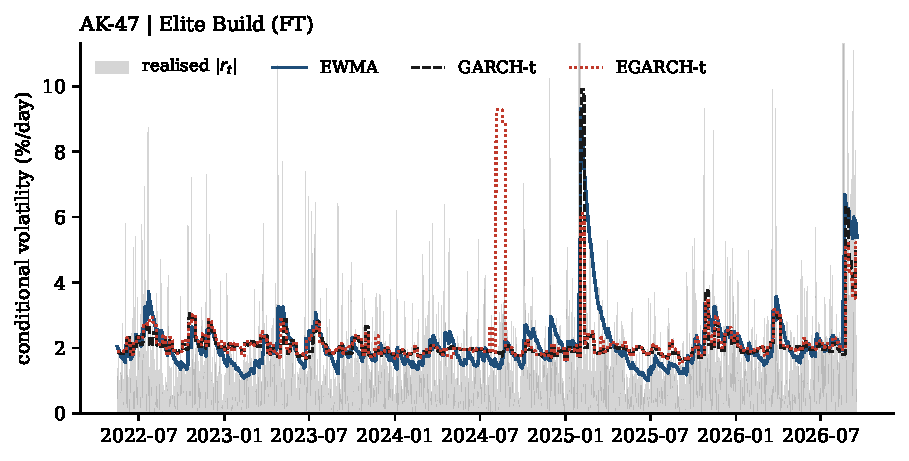
\includegraphics[width=\textwidth]{figures/fig4_forecasts}
\caption{Rolling one-day-ahead conditional volatility forecasts against
realised absolute returns for a representative item. The estimated
specifications track the realised series no more closely than the
parameter-free benchmark.}
\label{fig:forecasts}
\end{figure}

\paragraph{Robustness to the mean specification.}
Because AR(7) improves in-sample fit substantially
(Table~\ref{tab:mean}), we verified that it does not alter the forecast
ranking. On the three longest series, mean QLIKE under AR(7) is marginally
\emph{worse} than under AR(1) (2.885 against 2.874; 3.127 against 3.085;
4.008 against 3.985), and EWMA beats both in every case. The conditional mean
contributes negligibly to one-step-ahead conditional variance, so a better mean
model does not produce better variance forecasts. This is a second instance of
the paper's central pattern: improved in-sample specification without
out-of-sample gain.

\paragraph{Interpretation.}
EWMA with $\lambda = 0.94$ implies a shock half-life of 11.2 days; fitted GARCH
half-lives in this panel run from 3 to 11 days. A model that is already in
approximately the right range without estimating anything outperforms one that
must locate that range from a 500-day window spanning multiple regimes. Read
alongside the eight boundary solutions of Section~\ref{sec:models}, the picture
is of series carrying too little stable second-moment structure to support
estimating three variance parameters.

\subsection{Model confidence set}

Diebold--Mariano is a pairwise test. With five models there are ten
comparisons per item, and testing all ten at the 5\% level without correction
gives roughly a 40\% chance of at least one spurious rejection. We therefore
also apply the Model Confidence Set of \citet{HLN2011}, which starts from the
full model set and sequentially eliminates specifications that are
significantly worse, returning the subset that cannot be statistically
separated from the best. We use a 90\% set, a stationary bootstrap with 1{,}000
replications, and a block length of ten to accommodate autocorrelated loss
differentials.

\begin{table}[htbp]
\centering
\caption{Inclusion in the 90\% Model Confidence Set, 19 items}
\label{tab:mcs}
\begin{tabular}{lcc}
\toprule
Model & Items included & Share \\
\midrule
EWMA        & \textbf{19} & \textbf{100.0\%} \\
EGARCH-$t$  & 11 & 57.9\% \\
GARCH-$t$   & 11 & 57.9\% \\
GJR-$t$     & 11 & 57.9\% \\
Rolling SD  & 9  & 47.4\% \\
\bottomrule
\end{tabular}
\end{table}

EWMA is never eliminated. Each estimated specification survives on 11 of 19
items and is excluded on the remaining 8; on 7 items \emph{every} estimated
specification is excluded simultaneously. Five items yield a singleton
confidence set, and in every case the sole survivor is EWMA.

The MCS result is more informative than the pairwise tests in both directions.
It is stronger in that EWMA is the only model never excluded and the only model
ever to survive alone. It is weaker, and this should be stated plainly, in that
on 11 of 19 items the estimated specifications cannot be distinguished from
EWMA at all: the claim is not that GARCH is reliably worse everywhere, but that
it is never better and is sometimes demonstrably worse.

\subsection{Sensitivity to cleaning choices}

The repair thresholds and price floor of Section~\ref{sec:data} were selected
by inspection, which invites the objection that the result is an artefact of
those choices. We re-ran the full pipeline---cleaning, estimation, rolling
forecasts and comparison---on the eight longest series under four settings,
including one in which the spike-repair filter is disabled entirely.

\begin{table}[htbp]
\centering
\caption{Mean QLIKE under alternative cleaning specifications, 8 items}
\label{tab:robust}
\begin{tabular}{lccccc}
\toprule
Setting & EWMA & Rolling SD & GARCH-$t$ & EGARCH-$t$ & GJR-$t$ \\
\midrule
Loose (0.60 / 0.25 / RM 0.25)  & \textbf{3.844} & 3.906 & 4.048 & 4.088 & 4.065 \\
Baseline (0.80 / 0.35 / RM 0.50) & \textbf{3.852} & 3.917 & 4.057 & 4.102 & 4.075 \\
Strict (1.00 / 0.45 / RM 1.00) & \textbf{3.871} & 3.931 & 4.080 & 4.143 & 4.098 \\
No repair                      & \textbf{4.032} & 4.125 & 4.491 & 4.650 & 4.537 \\
\bottomrule
\end{tabular}
\end{table}

EWMA beats every estimated specification on all eight items under all four
settings---32 of 32 cases. The ordering of models is identical throughout.

One feature of Table~\ref{tab:robust} is worth drawing out. Disabling the
repair filter raises losses for every model, but it raises them far more for
the estimated specifications (GARCH-$t$ from 4.057 to 4.491) than for EWMA
(3.852 to 4.032). Isolated bad prints damage maximum-likelihood estimation more
than they damage a fixed-decay recursion. Our cleaning therefore works
\emph{against} the paper's central result: a reader who believes the repair
step is too aggressive should note that removing it widens the gap rather than
closing it.

\subsection{\texorpdfstring{Sensitivity to $\lambda$}{Sensitivity to lambda}}

If $\lambda = 0.94$ merely happened to suit this data, the result would be a
coincidence rather than evidence about estimation. We therefore re-ran EWMA
across a grid spanning a sixteen-fold range of decay speeds and re-tested each
against the same estimated forecasts (Table~\ref{tab:lambda}).

\begin{table}[htbp]
\centering
\caption{EWMA performance across smoothing constants}
\label{tab:lambda}
\begin{tabular}{lccc}
\toprule
$\lambda$ & Implied half-life & Mean QLIKE & DM losses to any estimated model \\
\midrule
0.85 & 4.3 days  & 3.766 & 0 / 57 \\
0.90 & 6.6 days  & 3.727 & 0 / 57 \\
0.94 & 11.2 days & 3.710 & 0 / 57 \\
0.97 & 22.8 days & 3.722 & 0 / 57 \\
0.99 & 69.0 days & 3.758 & 0 / 57 \\
\bottomrule
\end{tabular}
\end{table}

Every value of $\lambda$ yields mean QLIKE below the best estimated
specification (3.917), and EWMA loses no Diebold--Mariano test to any estimated
model at any $\lambda$. The advantage is therefore not an artefact of the
smoothing constant.

The claim should nonetheless be stated precisely. EWMA does lose to the rolling
standard deviation benchmark on one item at $\lambda = 0.85$ and one at
$\lambda = 0.99$, at the extremes of the grid. The defensible statement is that
no estimated GARCH-family specification beats a parameter-free benchmark, and
that EWMA's advantage over estimated models is insensitive to $\lambda$---not
that EWMA is uniformly superior.

%=======================================================================
\section{The 23 October 2025 supply shock}\label{sec:shock}
%=======================================================================

On 23 October 2025 Valve extended the Trade-Up Contract mechanism to permit
exchanging five Covert-quality skins for a knife or gloves, ending the supply
bottleneck that had supported knife prices since the market's inception.
Table~\ref{tab:shock} reports the effect on panel items over the following
five days.

\begin{table}[htbp]
\centering
\caption{Price change around the Trade-Up policy change, 22--27 October 2025}
\label{tab:shock}
\begin{tabular}{llr}
\toprule
Item & Tier & Change \\
\midrule
$\bigstar$ Flip Knife $\vert$ Doppler (FN)            & Above RM 500 & $-43\%$ \\
$\bigstar$ Bayonet $\vert$ Doppler (FN)               & Above RM 500 & $-39\%$ \\
$\bigstar$ Shadow Daggers $\vert$ Gamma Doppler (FN)  & Above RM 500 & $-29\%$ \\
AWP $\vert$ Chromatic Aberration (FT)                 & RM 50--500   & $+378\%$ \\
AK-47 $\vert$ Head Shot (FT)                          & RM 50--500   & $+394\%$ \\
\bottomrule
\end{tabular}
\end{table}

\begin{figure}[htbp]
\centering
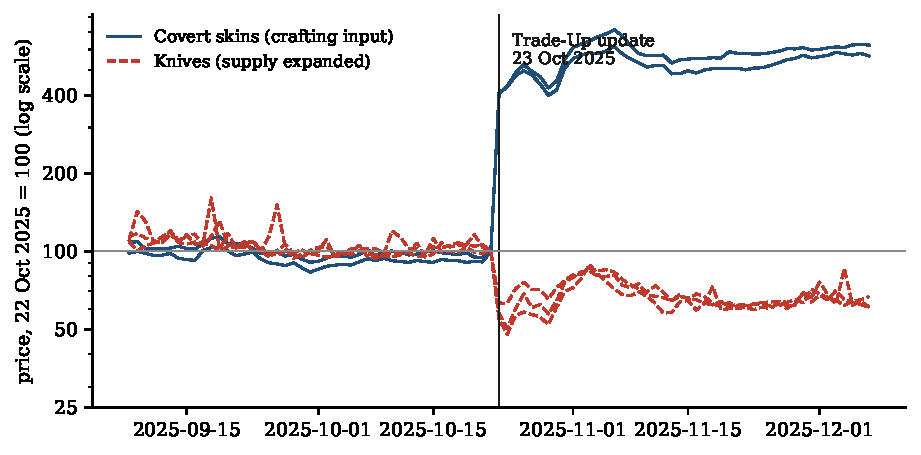
\includegraphics[width=\textwidth]{figures/fig5_shock}
\caption{Normalised price paths around the Trade-Up policy change, rebased to
22 October 2025. Covert skins, which became a crafting input, rose roughly
four-fold; knives, whose supply constraint was removed, fell by 30--45\%.
Log scale.}
\label{fig:shock}
\end{figure}

The episode provides a dated, exogenous, opposite-signed supply shock with
natural treatment and control groups. We partition the panel into three:
\emph{treated} (two Covert skins that became a crafting input), \emph{supply}
(three knives whose supply constraint was removed), and \emph{control}
(fifteen remaining items).

\subsection{Design}

Every specification is estimated once on the 500 trading days ending 22 October
2025 and then filtered forward through the event with parameters held fixed.
This is a test of parameter staleness rather than of re-estimation, and it is
fair across model classes: each model continues to update its conditional
variance recursively as returns arrive---GARCH through its recursion, EWMA
through its decay---so the only difference is how much each had to learn in the
first place. Losses are QLIKE, as in Section~\ref{sec:forecast}. Baseline is
mean loss over the 250 days preceding the event; recovery is the first day on
which a twenty-day rolling mean loss returns to within 10\% of that baseline.

\subsection{Results}

\begin{table}[htbp]
\centering
\caption{QLIKE deterioration over the 20 days following the shock, and days to
recovery}
\label{tab:shockloss}
\begin{tabular}{llccccc}
\toprule
& & EWMA & GARCH-$t$ & EGARCH-$t$ & GJR-$t$ & Rolling SD \\
\midrule
\multirow{2}{*}{Control (15)} & deterioration & 2.69 & 2.94 & 2.96 & 3.06 & 3.15 \\
 & recovery (days) & 32.1 & 30.3 & 29.7 & 30.4 & 33.2 \\[0.3em]
\multirow{2}{*}{Supply (3)} & deterioration & 2.59 & 2.56 & 2.61 & 2.66 & 2.83 \\
 & recovery (days) & 20.0 & 20.3 & 20.0 & 20.7 & 20.0 \\[0.3em]
\multirow{2}{*}{Treated (2)} & deterioration & 111.9 & 105.0 & 114.8 & 52.2 & 112.5 \\
 & recovery (days) & --- & 41.0 & 39.5 & 38.5 & 50.0 \\
\bottomrule
\end{tabular}
\end{table}

Three findings.

\paragraph{Deterioration is uniform across specifications.}
For the control and supply groups, QLIKE rises by 2.6 to 3.2 regardless of
model, and recovery takes 20 to 33 days. No specification degrades
meaningfully less than any other, and---consistent with
Section~\ref{sec:forecast}---the parameter-free EWMA is marginally best in the
control group. Estimated models do not have more to unlearn, because they did
not have much to know.

\paragraph{The apparent GJR advantage is an artefact.}
GJR-$t$ shows roughly half the deterioration of every other specification on
treated items (52.2 against 105--115), which would ordinarily be read as
asymmetry providing protection. It is not. Figure~\ref{fig:shockloss} shows
the daily loss path: essentially the entire deterioration is a single
observation. On the event day itself, QLIKE reaches between 780 and 2{,}900
depending on specification; by the following day every model is back to 6--9.
GJR's advantage consists of having entered that one day with a higher
conditional variance level than its competitors, on two items. This is a
single-day difference on an $n$ of two, and it should not be interpreted as
evidence about asymmetric specifications.

\begin{figure}[htbp]
\centering
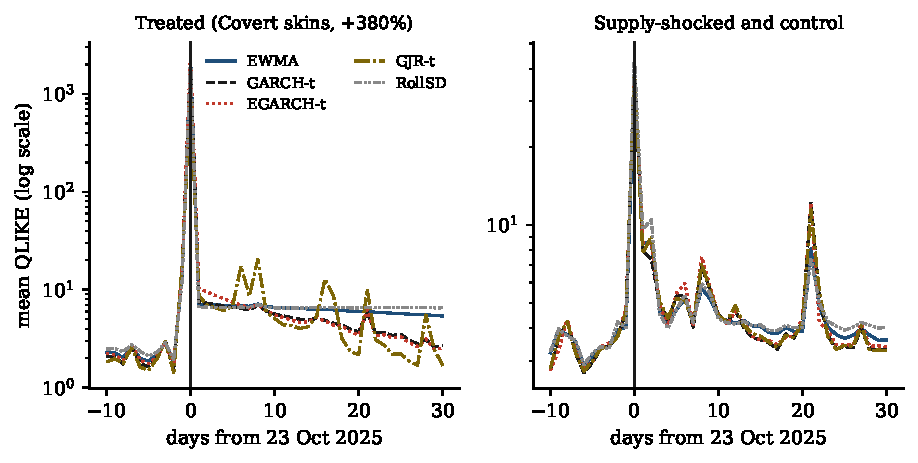
\includegraphics[width=\textwidth]{figures/fig6_shock_losses}
\caption{Mean daily QLIKE around 23 October 2025, log scale. The treated-group
deterioration is concentrated almost entirely in the event day itself.}
\label{fig:shockloss}
\end{figure}

\paragraph{EWMA's memory is a liability at the tail.}
Fifteen of 100 item--model pairs fail to recover within 60 days, and EWMA
accounts for five of them---more than any other specification, and it never
recovers on the treated group at all. The mechanism is the one that makes EWMA
attractive elsewhere: an infinite geometric memory means a single extreme
squared return persists in the recursion indefinitely, whereas a mean-reverting
GARCH recursion pulls back towards its unconditional level. This is the one
dimension on which the estimated models outperform.

\subsection{Interpretation}

The honest summary is that no specification offers meaningful protection
against a shock of this magnitude. Forecast losses on directly affected items
rise by a factor of forty on the event day and no model anticipates or absorbs
it. What differentiates the models is not robustness to the shock but behaviour
afterwards, where mean reversion in the GARCH recursion is an advantage that
EWMA lacks.

We note the obvious limitation: two treated items and three supply-shocked
items. Nothing in this section is well powered, and the results are reported as
description of a single episode rather than as tests.

%=======================================================================
\section{Limitations}
%=======================================================================

\begin{itemize}
\item \textbf{Small cross-section.} Twenty-two items in the main panel, with as
few as one in a price tier after exclusions. Cross-sectional claims are
presented as patterns, not tests.

\item \textbf{Tier and event are confounded.} Knives constitute both the
highest price tier and the principal casualty of the October 2025 shock, so the
persistence and event analyses are not cleanly separable.

\item \textbf{Noisy volatility proxy.} Squared daily returns rather than
realised variance. QLIKE mitigates but does not eliminate the resulting
inference problem, and results are not directly comparable to studies using
intraday data.

\item \textbf{Error distribution.} Estimated $\nu$ below 4 on most items means
the fitted $t$ has undefined kurtosis; standardised residual kurtosis of 6--8
indicates remaining unmodelled tail behaviour. Skewed-$t$ and GED
alternatives are untested.

\item \textbf{Unequal samples.} Item histories range from roughly 500 to 2{,}086
observations over 2021--2026, so items are estimated across different market
regimes.

\item \textbf{Survivorship.} Selection on liquidity measured over full history
favours items that remained liquid; items that became illiquid are absent by
construction.

\item \textbf{Single venue.} Steam Community Market only. Third-party
marketplaces carry substantial volume at different prices.

\item \textbf{Sensitivity analysis is partial.} The cleaning robustness check
covers the eight longest series rather than the full panel, for runtime
reasons, and varies the repair thresholds jointly rather than one at a time.

\item \textbf{Seasonal specification.} AR(7) is a blunt instrument for a
weekday effect: it spends seven parameters where day-of-week dummies would
spend six and target the effect directly. Residual lag-7 autocorrelation
remains significant on 13 of 22 items, indicating the seasonal is not fully
captured.

\item \textbf{Benchmark set.} EWMA is compared against estimated models only.
A wider set of parameter-free benchmarks would strengthen the claim.
\end{itemize}

%=======================================================================
\section{Conclusion}
%=======================================================================

The CS2 skin market has genuine conditional heteroskedasticity: volatility
clusters, returns are heavily fat-tailed, and ARCH tests reject on almost every
item. It nonetheless resists the standard technology for exploiting that
structure. No estimated GARCH-family specification improves on a
parameter-free benchmark out of sample on any item in our panel, and the
specification that fits best in sample forecasts worst out of it.

The claim survives the obvious challenges. An exponentially weighted average
lies inside the 90\% Model Confidence Set on every item and alone on five,
while estimated specifications are excluded outright on seven. The ranking is
unchanged across a sixteen-fold range of smoothing constants and across four
cleaning specifications, including one with no outlier repair at all---under
which the gap in fact widens.

We read this as a statement about the market rather than about the models.
Volatility shocks here decay with half-lives of days rather than weeks;
supply can be altered by decree without warning; and a third of items sit at or
near the boundary of integrated volatility. Under those conditions, estimating
three conditional variance parameters from a rolling window is a poor
allocation of the available information, and a fixed decay rate in
approximately the right range does better. That a market can display strong
volatility clustering and still defeat volatility models is, we think, the more
interesting finding.

Two further results deserve emphasis. The conditional mean is predictable on
every item, with a weekly cycle that no equity market would sustain, and the
panel exhibits both classical microstructure signatures simultaneously---
bid--ask bounce among high-value items, stale pricing among cheap ones---
separated cleanly by price. Taken together these describe a market whose
observable dynamics are dominated by frictions and participation patterns
rather than by the arrival of information, which is precisely the setting in
which conditional variance models have least to offer.

%=======================================================================
\begin{thebibliography}{99}

\bibitem[Amihud(2002)]{Amihud2002}
Amihud, Y. (2002).
\newblock Illiquidity and stock returns: cross-section and time-series effects.
\newblock \emph{Journal of Financial Markets}, 5(1), 31--56.

\bibitem[Andersen and Bollerslev(1998)]{AndersenBollerslev1998}
Andersen, T. G. and Bollerslev, T. (1998).
\newblock Answering the skeptics: yes, standard volatility models do provide
accurate forecasts.
\newblock \emph{International Economic Review}, 39(4), 885--905.

\bibitem[Bollerslev(1986)]{Bollerslev1986}
Bollerslev, T. (1986).
\newblock Generalized autoregressive conditional heteroskedasticity.
\newblock \emph{Journal of Econometrics}, 31(3), 307--327.

\bibitem[Diebold and Mariano(1995)]{DieboldMariano1995}
Diebold, F. X. and Mariano, R. S. (1995).
\newblock Comparing predictive accuracy.
\newblock \emph{Journal of Business \& Economic Statistics}, 13(3), 253--263.

\bibitem[Dobrynskaya and Strelnikov(2025)]{Dobrynskaya2025}
Dobrynskaya, V. and Strelnikov, V. (2025).
\newblock Videogame attributes as alternative investments.
\newblock \emph{Quarterly Journal of Finance}, 15(4), 1--22.

\bibitem[Engle(1982)]{Engle1982}
Engle, R. F. (1982).
\newblock Autoregressive conditional heteroscedasticity with estimates of the
variance of United Kingdom inflation.
\newblock \emph{Econometrica}, 50(4), 987--1007.

\bibitem[Glaser(2022)]{Glaser2022}
Glaser, T. (2022).
\newblock Steam and the platformization of virtual goods: an analysis of the
weapon skin economy in Counter-Strike: Global Offensive.
\newblock \emph{Spiel$\vert$Formen}, 2022, 139--162.

\bibitem[Glosten et al.(1993)]{Glosten1993}
Glosten, L. R., Jagannathan, R. and Runkle, D. E. (1993).
\newblock On the relation between the expected value and the volatility of the
nominal excess return on stocks.
\newblock \emph{Journal of Finance}, 48(5), 1779--1801.

\bibitem[Gu(2026)]{Gu2026}
Gu, X. (2026).
\newblock Speculative bubbles and liquidity crises in unregulated virtual
economies: an empirical analysis based on the CS:GO/CS2 skin market.
\newblock SSRN working paper 6482540.

\bibitem[Hansen and Lunde(2005)]{HansenLunde2005}
Hansen, P. R. and Lunde, A. (2005).
\newblock A forecast comparison of volatility models: does anything beat a
GARCH(1,1)?
\newblock \emph{Journal of Applied Econometrics}, 20(7), 873--889.

\bibitem[Hansen et al.(2011)]{HLN2011}
Hansen, P. R., Lunde, A. and Nason, J. M. (2011).
\newblock The model confidence set.
\newblock \emph{Econometrica}, 79(2), 453--497.

\bibitem[Harvey et al.(1997)]{Harvey1997}
Harvey, D., Leybourne, S. and Newbold, P. (1997).
\newblock Testing the equality of prediction mean squared errors.
\newblock \emph{International Journal of Forecasting}, 13(2), 281--291.

\bibitem[Lamoureux and Lastrapes(1990)]{LamoureuxLastrapes1990}
Lamoureux, C. G. and Lastrapes, W. D. (1990).
\newblock Persistence in variance, structural change, and the GARCH model.
\newblock \emph{Journal of Business \& Economic Statistics}, 8(2), 225--234.

\bibitem[Lo and MacKinlay(1990)]{LoMacKinlay1990}
Lo, A. W. and MacKinlay, A. C. (1990).
\newblock An econometric analysis of nonsynchronous trading.
\newblock \emph{Journal of Econometrics}, 45(1--2), 181--211.

\bibitem[Nelson(1991)]{Nelson1991}
Nelson, D. B. (1991).
\newblock Conditional heteroskedasticity in asset returns: a new approach.
\newblock \emph{Econometrica}, 59(2), 347--370.

\bibitem[Nikolaenko(2025)]{Nikolaenko2025}
Nikolaenko, A. (2025).
\newblock Time-series analysis of CS:GO/CS2 skin prices: stationarity, breaks,
and volatility forecasting.
\newblock Working paper, December 2025. Available via ResearchGate.

\bibitem[Nian(2026)]{Nian2026}
Nian, Z. (2026).
\newblock The application of event study method in virtual goods markets:
based on CS:GO skin prices.
\newblock \emph{Frontiers in Economics and Management}, 7(1), 69--85.

\bibitem[Newey and West(1987)]{NeweyWest1987}
Newey, W. K. and West, K. D. (1987).
\newblock A simple, positive semi-definite, heteroskedasticity and
autocorrelation consistent covariance matrix.
\newblock \emph{Econometrica}, 55(3), 703--708.

\bibitem[Patton(2011)]{Patton2011}
Patton, A. J. (2011).
\newblock Volatility forecast comparison using imperfect volatility proxies.
\newblock \emph{Journal of Econometrics}, 160(1), 246--256.

\bibitem[Roll(1984)]{Roll1984}
Roll, R. (1984).
\newblock A simple implicit measure of the effective bid--ask spread in an
efficient market.
\newblock \emph{Journal of Finance}, 39(4), 1127--1139.

\bibitem[Scholes and Williams(1977)]{ScholesWilliams1977}
Scholes, M. and Williams, J. (1977).
\newblock Estimating betas from nonsynchronous data.
\newblock \emph{Journal of Financial Economics}, 5(3), 309--327.

\bibitem[RiskMetrics(1996)]{RiskMetrics1996}
J.P. Morgan and Reuters (1996).
\newblock \emph{RiskMetrics Technical Document}, 4th edition.
\newblock New York.

\end{thebibliography}

\end{document}
